\chapter{Current peak transducer}
\section{Theory and related work} \label{sec:literature_current}
A current transducer converts the current flowing through some part of a circuit to a DC voltage output. From this definition, it is clear to see that its operation will mimic that of the voltage peak transducer implemented in Section \ref{sec:literature_voltage}. An AC voltage signal can be obtained by using a current sense resistor (that is small enough to have negligible effect on the voltage and current through the load). This can now serve as the input to a modified voltage transducer.

The precision rectifier shown in Figure \ref{subfig:superdiode} is used as part of a peak detector circuit. This is combined with a non-inverting amplifier, shown in Figure \ref{fig:non_invert_amp}\cite{non_invert_amp}. This reduces the gain needed for the output amplification stage. Thus, the influence of noise (especially ripple voltage) through the peak detector is minimised in the output. As this project requires the entire current input spectrum to be mapped, a standard non-inverting amplifier can be used instead of the difference amplifier previously used.

\begin{figure}
        \centering
         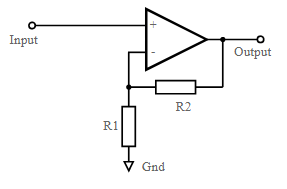
\includegraphics[width=0.35\linewidth]{./Figures/non_invert_amplifier}
		    \caption{Non-inverting amplifier\cite{non_invert_amp}} \label{fig:non_invert_amp}
 \end{figure}
 
\section{Design} \label{sec:design_current}
The first consideration for the transducer is what size of current sense resistor to use. Two are provided: a $\SI{5}{\milli\ohm}$ and a $\SI{30}{\milli\ohm}$. The larger resistor is chosen as it will provide larger input voltages for the same current, while still being much smaller than the maximum sized load ($\SI{100}{\ohm}$.

The peak detector is designed to also amplify the input voltage peak. The gain is chosen to be large enough that the output gain stage is relatively small, but small enough as to not exceed the output op-amp limits. The maximum common-mode input is $\SI{3.5}{\volt}$. Ideally, we would want the output gain to be less than 10. So: $53.33 \leq Gain \leq 388.89$. A gain of 181 is chosen, using $\SI{180}{\kilo\ohm}$ and $\SI{1}{\kilo\ohm}$ resistors.

With this gain, the output gain can be calculated by mapping $\SI{285}{\milli\ampere}$ to $\SI{4.5}{\volt}$. This gives a gain of 2.9078. $Gain = 1 + \frac{R_2}{R_1}$ from Figure \ref{fig:non_invert_amp}. Setting $R_2$ as $\SI{5.6}{\kilo\ohm}$ and $R_1$ as $\SI{3.3}{\kilo\ohm}$ gives a gain of 2.7 which is sufficient.

The capacitor value for the peak detector is chosen, as before, to produce ripple less than the change expected for accuracy of the transducer. In this case, $\SI{1}{\milli\ampere}$ is required, so the capacitor is obtained as follows\cite{Neamen:Microelectronics}:
\begin{equation}
\begin{split}
    V_r &= \SI{1}{\milli} \times \SI{30}{\milli} \times 181 = \SI{5.43}{\milli\volt} \\
    V_r &= \frac{V_{pk}}{fRC} \\
    C &= \frac{\SI{285}{\milli} \times \SI{30}{\milli} \times 181}{\SI{5.43}{\milli} \times 1M \times 50} \\
    &= \SI{5.7}{\mu\farad} \\
\end{split}
\end{equation}
Once again, for maximum accuracy during sampling, a capacitor ten times larger is chosen. Thus, a $\SI{47}{\mu\farad}$ capacitor is used.

As a 10-bit ADC is to be used, the resolution is given as 4.883mV/bit. Reversing this to the input of the transducer gives a resolution of $\SI{10}{\mu\volt}$/bit or $\SI{0.3334}{\milli\ampere}$/bit. This is less than our specified accuracy, but close enough as to affect the accuracy of the transducer.

The complete current peak transducer circuit is provided in Figure \ref{fig:current_circuit}.

\begin{figure}
        \centering
         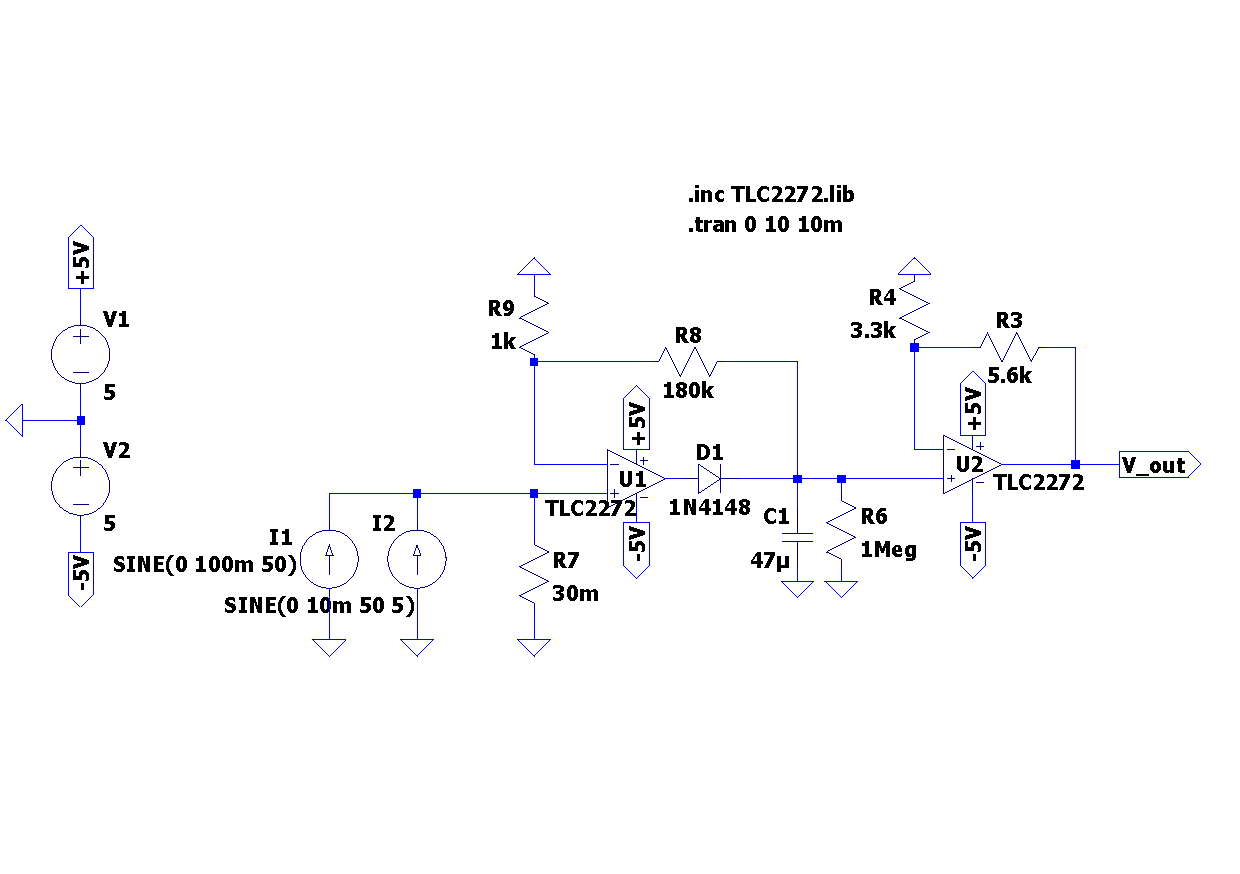
\includegraphics[width=1\linewidth]{./Figures/current_circuit.pdf}
		    \caption{Current transducer circuit.} \label{fig:current_circuit}
 \end{figure}

\section{Simulation} \label{sec:simulation_current}

\begin{figure}
        \centering
         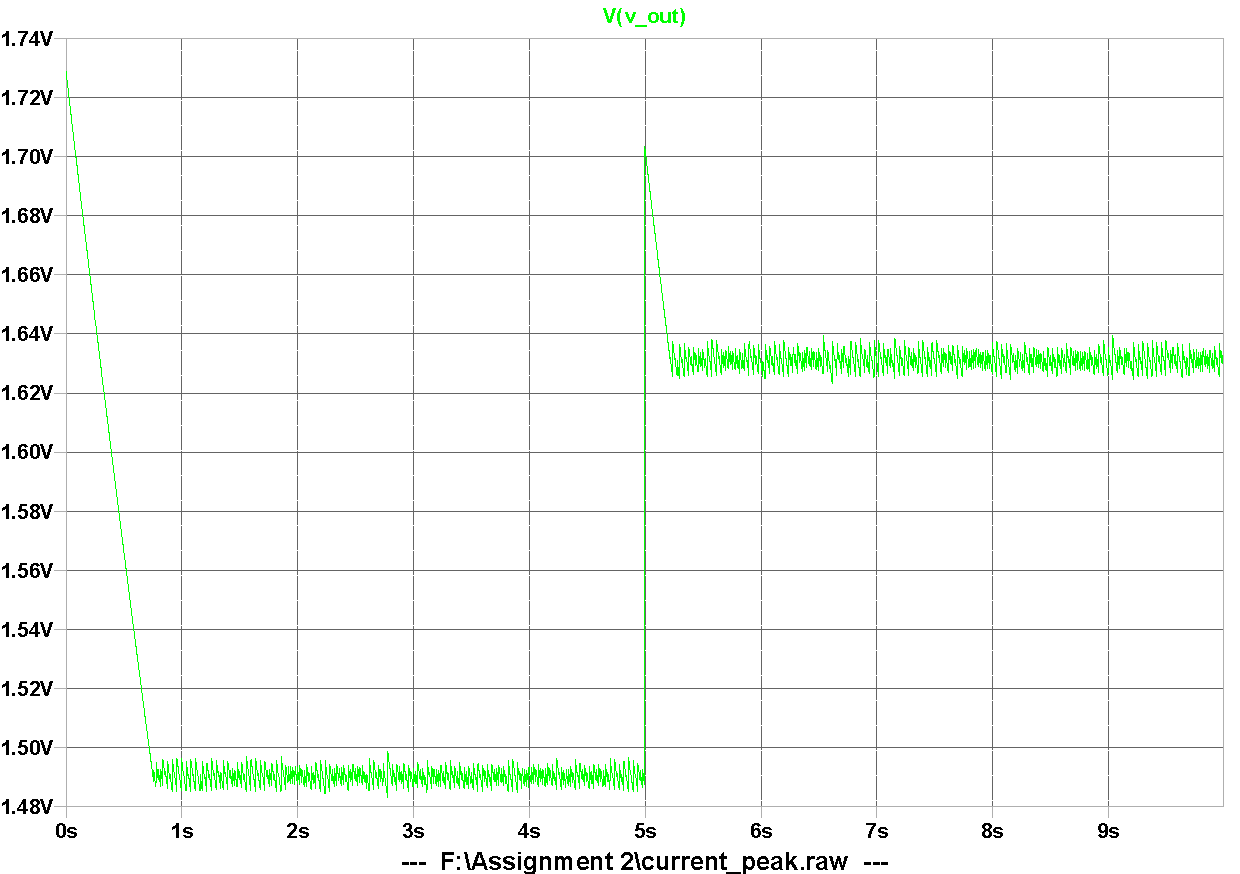
\includegraphics[width=0.75\linewidth]{./Figures/current_transducer_simulation.pdf}
		    \caption{Current transducer simulation.} \label{fig:current_simulate}
 \end{figure}
 
 
\section{Measurements} \label{sec:measurements_current}
The deduced input in Tables \ref{tab:current_unit_test} and \ref{tab:current_integrated_test} is derived from the circuit in Figure \ref{fig:current_circuit}.

$V_{out} = (1+\frac{5.6k}{3.3k}) \times 181 \times 30\si{\milli} \times I = I(14.6445)$
\begin{figure}
 \centering
     \begin{subfigure}[]{0.45\textwidth}
        \centering
         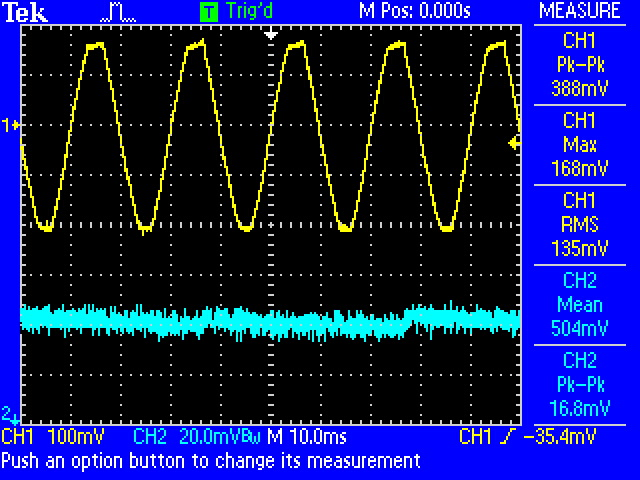
\includegraphics[width=1\linewidth]{./Figures/current_measure}
		    \caption{AC input and DC output for mid range load.} \label{subfig:current_measure}
     \end{subfigure}
      \begin{subfigure}[]{0.45\textwidth}
              \centering
  		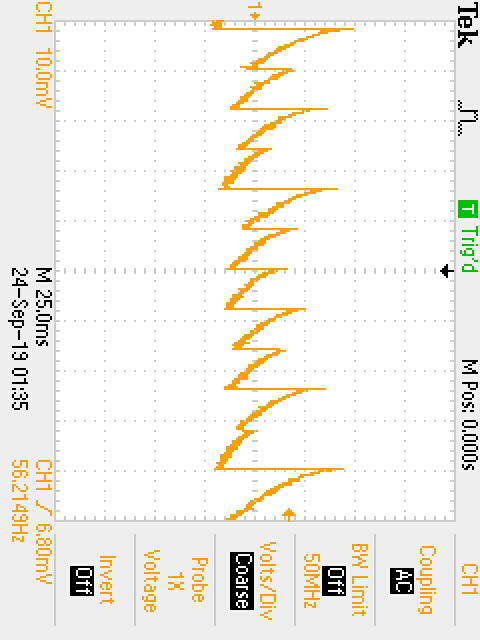
\includegraphics[height=1\linewidth,angle=90]{./Figures/current_noise_measure}
		    \caption{Current transducer noise levels for a mid sized load.} \label{subfig:current_noise}
     \end{subfigure}
 \end{figure}
 
\begin{table}[h]
        \centering
        \footnotesize
        \caption{Current transducer unit test results}
         \begin{tabular}{ccccccc}
          \toprule
             \textit{\footnotesize Emulated level} & \textit{\footnotesize Signal generator} & \textit{\footnotesize Signal generator} & \textit{{\footnotesize Analogue output}} & \textit{\footnotesize Deduced input} & \textit{\footnotesize Difference}\\
             $[VmA_{peak}]$ & $[mV]$ & $[mV]$ & $[\si{\volt}DC]$ & $[mA_{peak}]$ & $[mA]$ \\
          \hline
          0 & 0 & 3.84 & 0.115 & 7.853 & 7.853 \\
          50 & 16.5 & 19.4 & 0.780 & 53.26 & 3.26 \\
          100 & 33.0 & 36.4 & 1.52 & 103.79 & 3.79 \\
          101 & 33.3 & 36.6 & 1.53 & 104.47 & 3.47 \\
          102 & 33.7 & 37.2 & 1.55 & 105.84 & 3.84 \\
          200 & 66.0 & 69.8 & 3.00 & 204.85 & 4.85 \\
          285 & 94.0 & 98.0 & 4.27 & 291.57 & 6.57 \\
         \hline
        \end{tabular}
     \label{tab:current_unit_test}
\end{table}

\begin{table}[h]
        \centering
        \footnotesize
        \caption{Current transducer unit test results}
         \begin{tabular}{ccc|p{1.8cm}p{1.8cm}p{1.8cm}p{1.8cm}c}
          \toprule
             \textit{\footnotesize Measurement} & \textit{\footnotesize Load $R_1$} & \textit{\footnotesize Load $R_2$} & \textit{{\footnotesize Measured $\si{\volt}_R$}} & \textit{{\footnotesize Actual input}} & \textit{{\footnotesize Analogue output}} & \textit{\footnotesize Deduced input} & \textit{\footnotesize Difference}\\
             & $[\si{\ohm}]$ & $[\si{\ohm}]$ & $[mV_{peak}]$ & $[mA_{peak}]$ & $[\si{\volt}DC]$ & $[mA_{peak}]$ & $[mA]$ \\
          \hline
          No load & open & - & 43.4 & 7.993 & 0.114 & 7.78 & 0.213 \\
          Full load & 100 & - & 1620 & 298.34 & 4.35 & 297.04 & 1.30 \\
          Mid range & 1k & - & 199 & 36.648 & 0.499 & 34.074 & 2.574 \\
          Mid + $\delta$ & 1k & 24k & 207 & 38.12 & 0.516 & 35.235 & 2.885 \\
          Mid + $2\delta$ & 1k & 12k & 215 & 39.595 & 0.538 & 36.737 & 2.858 \\
          \hline
        \end{tabular}
     \label{tab:current_integrated_test}
\end{table}







